\documentclass[12pt,a4paper]{scrartcl}

%% (C) Hirnschall Sebastian 2016 

\usepackage{amsmath}% http://ctan.org/pkg/amsmath
\newcommand{\Mod}[1]{\ (\text{mod}\ #1)}

\usepackage[ngerman]{cleveref} %referenzen fur Abbildungen
\usepackage{graphicx}
\usepackage{listings}
\usepackage{color}
\usepackage{esdiff}
\usepackage[utf8]{inputenc}
\usepackage[ngerman]{babel}
\usepackage[T1]{fontenc}
\usepackage{amsmath}
\usepackage{graphicx}
\usepackage{amssymb}
\usepackage{geometry}% http://ctan.org/pkg/geometry



%\pagestyle{headings}

\bibliographystyle{plain}

\setcounter{secnumdepth}{5}
\setcounter{tocdepth}{5}

%\pagestyle{headings}

\usepackage{fancyhdr}
\pagestyle{fancy}
%
\rhead{ \leftmark}
\chead{}
\lhead{ \rightmark}
%%
\lfoot{ Sebastian Hirnschall}
\cfoot{}
\rfoot{\thepage}
%%
\renewcommand{\headrulewidth}{0.2pt}
\renewcommand{\footrulewidth}{0.2pt}


\fancypagestyle{firststyle}
{
   	\fancyhf{}
   	\lfoot{ Sebastian Hirnschall}
	\cfoot{}
	\rfoot{\thepage}
}


%listings settings
\definecolor{mygreen}{rgb}{0,0.6,0}
\definecolor{mygray}{rgb}{0.5,0.5,0.5}
\definecolor{mymauve}{rgb}{0.58,0,0.82}
\definecolor{BackgroundGray}{rgb}{0.9,0.9,0.9}

\lstset{ %
  backgroundcolor=\color{BackgroundGray},   % choose the background color; you must add \usepackage{color} or \usepackage{xcolor}
  basicstyle=\footnotesize,        % the size of the fonts that are used for the code
  breakatwhitespace=false,         % sets if automatic breaks should only happen at whitespace
  breaklines=true,                 % sets automatic line breaking
  captionpos=b,                    % sets the caption-position to bottom
  commentstyle=\color{mygreen},    % comment style
  deletekeywords={...},            % if you want to delete keywords from the given language
  escapeinside={\%*}{*)},          % if you want to add LaTeX within your code
  extendedchars=true,              % lets you use non-ASCII characters; for 8-bits encodings only, does not work with UTF-8
  frame=single,	                   % adds a frame around the code
  keepspaces=true,                 % keeps spaces in text, useful for keeping indentation of code (possibly needs columns=flexible)
  keywordstyle=\color{blue},       % keyword style
  language=C,                 	   % the language of the code
  otherkeywords={*,...},           % if you want to add more keywords to the set
  numbers=left,                    % where to put the line-numbers; possible values are (none, left, right)
  numbersep=5pt,                   % how far the line-numbers are from the code
  numberstyle=\tiny\color{mygray}, % the style that is used for the line-numbers
  rulecolor=\color{mygray},         % if not set, the frame-color may be changed on line-breaks within not-black text (e.g. comments (green here))
  showspaces=false,                % show spaces everywhere adding particular underscores; it overrides 'showstringspaces'
  showstringspaces=false,          % underline spaces within strings only
  showtabs=false,                  % show tabs within strings adding particular underscores
  stepnumber=2,                    % the step between two line-numbers. If it's 1, each line will be numbered
  stringstyle=\color{mymauve},     % string literal style
  tabsize=2,	                   % sets default tabsize to 2 spaces
  title=\lstname                   % show the filename of files included with \lstinputlisting; also try caption instead of title
}


%change title font
\usepackage{titlesec}
\titleformat*{\section}{\LARGE\bfseries}
\titleformat*{\subsection}{\Large\bfseries}
\titleformat*{\subsubsection}{\large\bfseries}
\titleformat*{\paragraph}{\large\bfseries}
\titleformat*{\subparagraph}{\large\bfseries}

\begin{document}
\newgeometry{bottom=1cm,top=1cm}
\begin{titlepage}
	\centering
	\begin{flushright}
		
\includegraphics[width=0.5\textwidth]{brgg-logo}\par\vspace{1cm}
	\end{flushright}	
		
	\vspace{4cm}
		
	{\scshape\huge \textbf{Vorwissenschaftliche Arbeit}\par}
	\vspace{1.5cm}
	Titel der Vorwissenschaftlichen Arbeit: \par
	\vspace{0.5cm}
	{\large\bfseries Funktionsweise und Schwachstellen von kryptographischen Hashfunktionen\par}
	\vspace{2cm}
	Verfasser: \par
	\vspace{0.3cm}
	{\Large \textbf{Sebastian Hirnschall}\par}
	\vfill
	\begin{flushleft}
		$ \, $ Wiener Neustadt, im Februar 2017 \par
		\begin{tabular}{l r}
			Klasse:     & 8AL           \\
			Fachgebiet: & Informatik    \\
			Schuljahr:  & 2016/2017     \\
			Betreuer:   & Dein Betreuer \\
		\end{tabular}
	\end{flushleft}
	
	
	
	% Bottom of the page
		
\end{titlepage}
\restoregeometry



\newpage
{\huge \bfseries Abstract}
\thispagestyle{firststyle}
	
\newpage
{\huge \bfseries Vorwort}
\thispagestyle{firststyle}

\newpage
\tableofcontents

\newpage
\section{Einleitung}
\newpage
\section{Hashfunktionen im Allgemeinen}
\subsection{Definition}
\begin{quote}
A hash function $H$ projects a value from a set with many (or even an infinite number of) members to a value from a set with a fixed number of (fewer) members. Hash functions are not reversible.\footnote{mathworld.wolfram.com/HashFunction.html}
\end{quote}

\noindent
Die Funktion $H$ bildet $A$ auf $B$ ab. Da die Menge $B$ weniger Element besitzt als $A$, handelt es sich bei Hashfunktionen um eine nicht injektive\footnote{$ f(x_1) = f(x_2) => x_1 = x_2$} Abbildung. %Siehe \cref{fig:nicht-injektive-abbildung}
	
\begin{figure}[!h]
	\vspace{0.5cm}
	\centering
	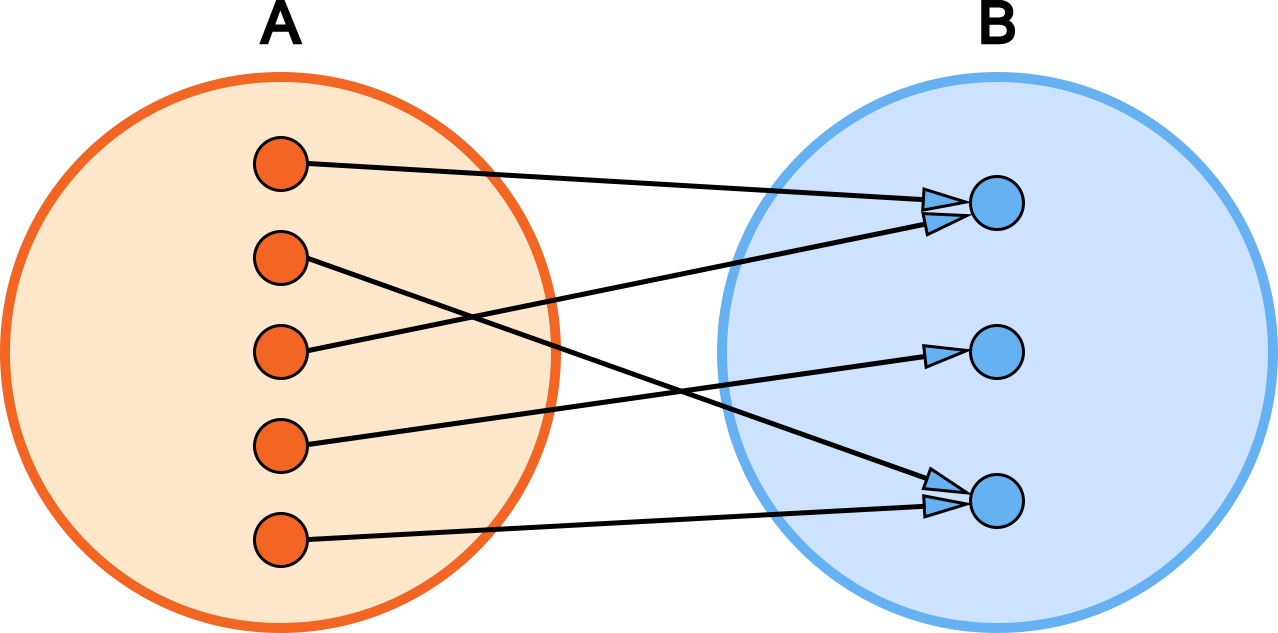
\includegraphics[width=0.7\textwidth]{nicht-injektive-abbildung}
	\caption[Caption for LOF]{nicht injektive Abbildung\footnotemark}
	\label{fig:nicht-injektive-abbildung}
\end{figure}
\footnotetext{erstellt von Sebastian Hirnschall}
	
\newpage
\subsection{Funktionsweise}
	
Um die Funktionsweise einer Hashfunktion zu verstehen, bretrachte man $H$.
\[ H(x)=y=\lfloor x \Mod{16} \rfloor \]
In diesem Beispiel werden alle $x\in \mathbb{R}$ auf $ \left\lbrace y \in \mathbb{N} \: | \: 0 \leq y \leq 16 \right\rbrace $ abgebildet. 	$\Rightarrow$	H(x) kann $2^4$ verschiedene Werte annehmen.
	
	
	
\begin{figure}[!h]
	\vspace{0.5cm}
	\centering
	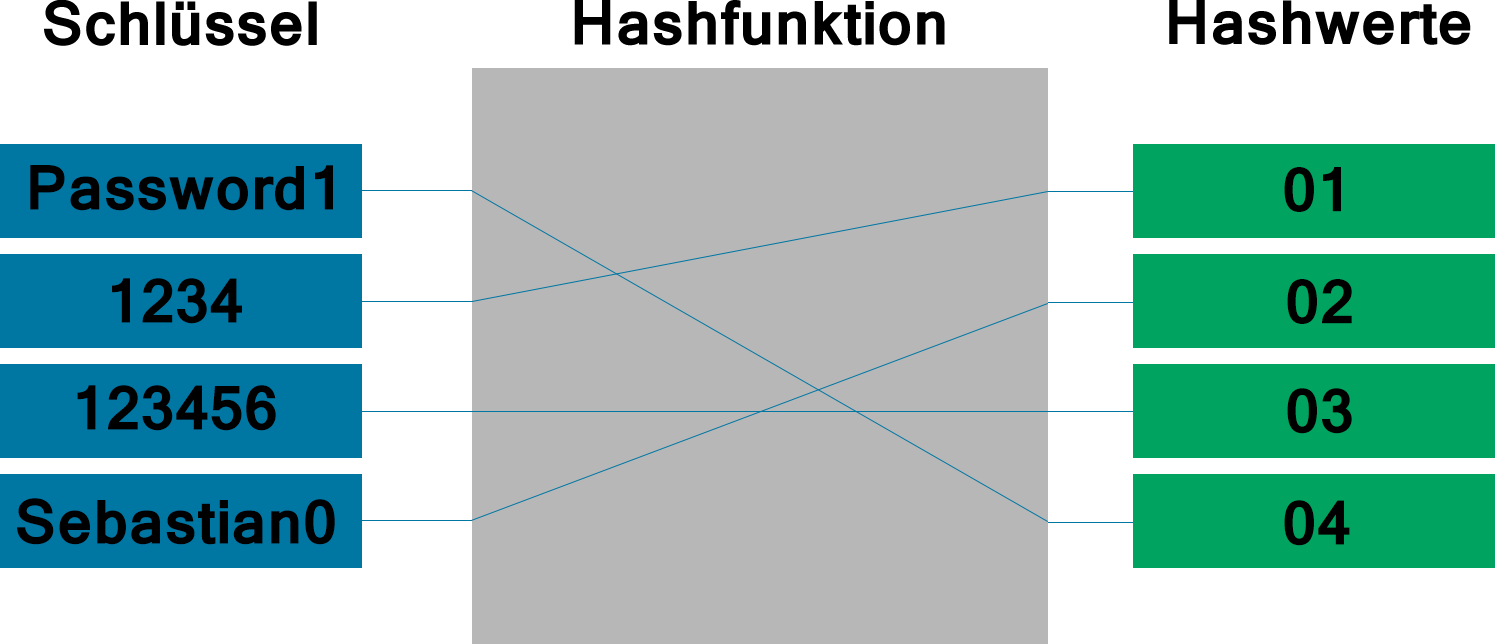
\includegraphics[width=0.7\textwidth]{hashfunktion}
	\caption[Caption for LOF]{Schema einer Hashfunktion\footnotemark}
	\label{fig:hashfunktion}
\end{figure}
\footnotetext{erstellt von Sebastian Hirnschall}
\newpage
\section{Bruteforce}
\lstinputlisting[language=c]{bruteforce.c}

\newpage

\end{document}
\end{flushleft}